\documentclass[12pt, a4paper]{article}
\usepackage[UTF8]{ctex} % 支持中文
\usepackage{amsmath, amssymb} % 数学公式
\usepackage{geometry} % 页面布局
\usepackage{fancyhdr} % 页眉页脚
\usepackage{xcolor} % 颜色
\usepackage{tcolorbox} % 文本框
\usepackage{enumitem} % 列表格式
\usepackage{tikz} % 绘图支持（用于题目12的图形）

% 页面设置：页边距适中，留出书写空间
\geometry{left=2.5cm, right=2.5cm, top=2.5cm, bottom=2.5cm}
\setlength{\headheight}{14.5pt} % 修复 fancyhdr 的 headheight 警告

% 页眉设置
\pagestyle{fancy}
\fancyhf{}
\fancyhead[L]{通信原理期末复习}
\fancyhead[R]{核心计算题突破}
\fancyfoot[C]{\thepage}

% 题目框样式
\newtcolorbox{problembox}[1]{
	colback=blue!5!white,
	colframe=blue!75!black,
	fonttitle=\bfseries,
	title={#1}
}

\title{\textbf{通信原理期末复习题集}\\ \large 核心计算题专项训练 (16题)}
\author{23届陈文斗}
\date{\today}

\begin{document}
	
	\maketitle
	\thispagestyle{empty}
	\begin{center}
		\vspace{1cm}
		\textbf{使用说明：}\\
		本题集包含16道典型计算题，涵盖了以下考点：\\
		\vspace{0.5cm}
		\begin{itemize}
			\item 八进制信源与误码率计算
			\item 高斯白噪声通过滤波器
			\item 香农公式与信道容量（含极限分析）
			\item 模拟调制 (AM / FM)
			\item 数字基带传输 (奈奎斯特准则 / M进制 / 传输可行性分析)
			\item PCM 信源编码 (TDM复用 / 占空比带宽 / 量化误差)
			\item 基带编码 (AMI / HDB3 码)
			\item 功率谱密度与调制方案选择
			\item 信息论应用 (图像传输 / 信息量计算)
		\end{itemize}
		\vspace{0.8cm}
		\textcolor{red}{\textbf{题目来源说明：}}\\
		\vspace{0.3cm}
		\begin{itemize}
			\item \textbf{题目 1-9}：期末考试真题回忆（实际考试题目）
			\item \textbf{题目 10-16}：根据考纲知识点补充的典型题
		\end{itemize}
	\end{center}
	\newpage
	
	% ==========================================
	% 题目 1
	% ==========================================
	\section*{题目 1：八进制离散信源与误码率计算}
	
	\begin{problembox}{已知条件}
		某数字通信系统传输 \textbf{八进制} 离散信源，\textbf{码元速率 $R_B=1200 \text{ Baud}$}，总传输码元数为 24000 个，错误码元数为 36 个。已知每个错误码元中，2/3 概率导致 3bit 信息错误，1/3 概率导致 1bit 信息错误（八进制符号每个携带 3bit 信息）。
	\end{problembox}
	
	\subsection*{求解：}
	\begin{enumerate}[label=(\arabic*)]
		\item 若各符号概率为 $P(x_1)=P(x_2)=1/4$， $P(x_3)=P(x_4)=1/8$， $P(x_5)=P(x_6)=P(x_7)=P(x_8)=1/16$，计算信源熵 $H(X)$；
		\item 计算系统信息速率 $R_b$；误码率 $P_e$；计算误信率 $P_b$；
		\item 若保持信息速率不变，改为二进制移相键控（2PSK，等概），计算新的码元速率 $R_B'$。
	\end{enumerate}
	
	\noindent\textbf{【解题区域 / 笔记】：}
	
	\newpage
	
	% ==========================================
	% 题目 2
	% ==========================================
	\section*{题目 2：高斯白噪声通过带通滤波器}
	
	\begin{problembox}{已知条件}
		中心频率为 $f_c=10^6 \text{ Hz}$、带宽 $B=4 \text{ kHz}$ 的理想带通滤波器，输入均值为 0、双边功率谱密度 $\frac{n_0}{2} = 2 \times 10^{-16} \text{ W/Hz}$ 的高斯白噪声。
	\end{problembox}
	
	\subsection*{求解：}
	\begin{enumerate}[label=(\arabic*)]
		\item 求输出噪声的功率谱密度和平均功率；
		\item 求输出噪声的一维概率密度函数。
	\end{enumerate}
	
	\noindent\textbf{【解题区域 / 笔记】：}
	
	\newpage
	
	% ==========================================
	% 题目 3 (更新版)
	% ==========================================
	\section*{题目 3：香农公式与信道容量}
	
	\begin{problembox}{已知条件}
		某 AWGN 信道，带宽 $B=10 \text{ kHz}$，噪声双边功率谱密度 $\frac{n_0}{2} = 5 \times 10^{-16} \text{ W/Hz}$，信号传输衰减系数为 20dB，发送端功率 $S_t=0.5 \text{ W}$。
	\end{problembox}
	
	\subsection*{求解：}
	\begin{enumerate}[label=(\arabic*)]
		\item 计算该系统的信道容量 $C$；
		\item \textbf{（简答）} 根据香农公式，简述在信道容量 $C$ 一定的情况下，带宽 $B$ 与信噪比 $S/N$ 之间的关系。并举例说明“以带宽换取信噪比”在通信系统中的应用；
		\item \textbf{（分析）} 为了提高容量，若无限增加带宽 $B$ ($B \to \infty$)，信道容量 $C$ 能否无限增加？请结合公式推导说明原因。
	\end{enumerate}
	
	\noindent\textbf{【解题区域 / 笔记】：}
	\textit{提示：(1) 注意 $S_t$ 是发送功率，计算信噪比需用接收功率 $S_r$；(3) 利用极限公式 $\lim_{x\to0} \ln(1+x)/x = 1$，极限容量 $C_{\infty} \approx 1.44 \frac{S}{n_0}$。}
	
	\newpage
	
	% ==========================================
	% 题目 4
	% ==========================================
	\section*{题目 4：AM 标准调幅分析}
	
	\begin{problembox}{已知条件}
		已知消息（调制）信号为 $m(t) = 3\cos(4000\pi t)$，载波信号为 $c(t) = 10\cos(4\pi \times 10^7 t)$。当采用正常调幅 AM 时。
	\end{problembox}
	
	\subsection*{求解：}
	\begin{enumerate}[label=(\arabic*)]
		\item 计算调幅系数 $m_a$；
		\item 写出已调 AM 信号的时域表达式；
		\item AM 信号的频域描述（画出频谱或写出表达式）；
		\item AM 信号的带宽；
		\item AM 信号的平均功率。
	\end{enumerate}
	
	\noindent\textbf{【解题区域 / 笔记】：}
	
	\newpage
	
	% ==========================================
	% 题目 5
	% ==========================================
	\section*{题目 5：FM 信号综合分析}
	
	\begin{problembox}{已知条件}
		已知 FM 信号的表达式为 $S_{FM}(t) = 10\cos(10^6\pi t + 8\cos 10^3\pi t) \text{ V}$，调频灵敏度 $K_f = 400\pi \text{ rad/(s}\cdot\text{V)}$。
	\end{problembox}
	
	\subsection*{求解：}
	\begin{enumerate}[label=(\arabic*)]
		\item 指出载波角频率和调制频率；
		\item 计算信号功率、调频指数和信号带宽；
		\item 写出相应的调制信号 $m(t)$ 表达式。
	\end{enumerate}
	
	\noindent\textbf{【解题区域 / 笔记】：}
	
	\newpage
	
	% ==========================================
	% 题目 6
	% ==========================================
	\section*{题目 6：FM 瞬时频率与参数变化}
	
	\begin{problembox}{已知条件}
		已知某单频调频波的振幅是 10V，瞬时频率 $f(t) = 10^6 + 10^4 \cos(2\pi \times 10^3 t) \text{ (Hz)}$。
	\end{problembox}
	
	\subsection*{求解：}
	\begin{enumerate}[label=(\arabic*)]
		\item 此调频波的表达式；
		\item 此调频波的最大频率偏移、调频指数和频带宽度；
		\item 若调制信号频率提高到 $2 \times 10^3 \text{ Hz}$，则调频波的频偏、调频指数和频带宽度如何变化？
		\item 若峰值频率偏移加倍，信息信号的幅度怎么变化？
	\end{enumerate}
	
	\noindent\textbf{【解题区域 / 笔记】：}
	
	\newpage
	
	% ==========================================
	% 题目 7
	% ==========================================
	\section*{题目 7：PCM 编码与复用带宽 (A律 vs 线性)}
	
	\begin{problembox}{已知条件}
		设某信号的带宽为 15-80KHz。
	\end{problembox}
	
	\subsection*{求解：}
	\begin{enumerate}[label=(\arabic*)]
		\item 编 A 律 13 折线 8 位码和线性 12 位码时的码元速率；
		\item 现将 10 路编 8 位码的该信号进行 PCM 时分复用传输，此时的码元速率为多少；
		\item 传输此时分复用 PCM 信号所需要的奈奎斯特基带带宽为多少。
	\end{enumerate}
	
	\noindent\textbf{【解题区域 / 笔记】：}
	
	\newpage
	
	% ==========================================
	% 题目 8
	% ==========================================
	\section*{题目 8：PCM 复用与占空比 (RZ vs NRZ)}
	
	\begin{problembox}{已知条件}
		对 10 路最高频率为 4kHz 的信号采用 PCM 时分复用传输，抽样后进行 8 级线性量化，并编为自然二进制码。码元波形为矩形脉冲，\textbf{占空比为 1}。
	\end{problembox}
	
	\subsection*{求解：}
	\begin{enumerate}[label=(\arabic*)]
		\item 传输此信号所需要的带宽；
		\item 若\textbf{占空比为 1/2}，重做 (1)。
	\end{enumerate}
	
	\noindent\textbf{【解题区域 / 笔记】：}
	\textit{提示：注意区分归零码(RZ)与不归零码(NRZ)的第一零点带宽差异。}
	
	\newpage
	
	% ==========================================
	% 题目 9
	% ==========================================
	\section*{题目 9：十六进制基带系统设计}
	
	\begin{problembox}{已知条件}
		某十六进制系统信道截止频率为 4000Hz，滚降系数 $\alpha=0.4$，满足奈奎斯特第一准则无码间干扰传输。
	\end{problembox}
	
	\subsection*{求解：}
	\begin{enumerate}[label=(\arabic*)]
		\item 最小传输带宽及符号间隔；
		\item 最大码元频带利用率；
		\item 最大信息频带利用率；
		\item 最大码元速率 $R_B$。
	\end{enumerate}
	
	\noindent\textbf{【解题区域 / 笔记】：}
	
	\newpage
	
	% ==========================================
	% 题目 10：PCM 量化误差与位数反推
	% ==========================================
	\section*{题目 10：PCM 量化误差与参数设计}
	
	\begin{problembox}{已知条件}
		设模拟信号的最高频率为 4kHz，若采用 PCM 方式进行传输，要求采用\textbf{均匀量化}，且\textbf{最大量化误差}为信号峰-峰值的 $0.25\%$。
	\end{problembox}
	
	\subsection*{求解：}
	\begin{enumerate}[label=(\arabic*)]
		\item 计算 PCM 信号的最低码元速率；
		\item 计算需要的奈奎斯特基带带宽；
		\item 若将其转换成 8 进制信号进行传输，此时的码元速率和需要的奈奎斯特基带带宽。
	\end{enumerate}
	
	\noindent\textbf{【解题区域 / 笔记】：}
	\textit{提示：量化误差 $ |e_{max}| \le \frac{\Delta}{2} $，需建立误差与量化级数 $M$ (或位数 $N$) 的不等式关系：$\frac{1}{2^{N+1}} \le 0.25\%$。}
	
	\newpage
	
	% ==========================================
	% 题目 11：基带传输可行性与系统设计
	% ==========================================
	\section*{题目 11：传输可行性分析与调制设计}
	
	\begin{problembox}{已知条件}
		一个带宽为 $0 \sim 1 \text{ MHz}$ 的信道，需要传输速率为 $3 \text{ Mb/s}$ 的\textbf{二进制}数字信号。
	\end{problembox}
	
	\subsection*{求解：}
	\begin{enumerate}[label=(\arabic*)]
		\item 判断该信道能否不失真传输此二进制信号，并说明理由；
		\item 若不能，设计一种采用\textbf{调制}的传输方式来解决此问题（需计算验证）；
		\item 画出你设计的传输方案的\textbf{收发端原理框图}。
	\end{enumerate}
	
	\noindent\textbf{【解题区域 / 笔记】：}
	\textit{提示：计算二进制所需的奈奎斯特带宽是否超过信道带宽。若超过，需采用 M 进制调制（如 4PSK/QPSK）以提高频带利用率。}
	
	\newpage
	
	% ==========================================
	% 题目 12：奈奎斯特准则的图形分析 (ISI 判定)
	% ==========================================
	\section*{题目 12：数字基带传输特性的图形分析}
	
	\begin{problembox}{已知条件}
		数字基带传输系统的传输特性 $H(\omega)$ 如下图所示（梯形谱）：
		\begin{center}
			% 简易示意图绘制
			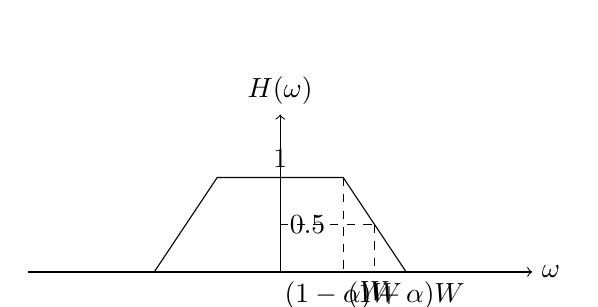
\begin{tikzpicture}[scale=0.8]
				\draw[->] (-4,0) -- (4,0) node[right] {$\omega$};
				\draw[->] (0,0) -- (0,2.5) node[above] {$H(\omega)$};
				\draw (-2,0) -- (-1,1.5) -- (1,1.5) -- (2,0);
				\node at (0,1.5) [above] {1};
				\node at (0,0.75) [right] {0.5};
				\draw[dashed] (1,1.5) -- (1,0) node[below] {$(1-\alpha)W$};
				\draw[dashed] (2,0) -- (2,0) node[below] {$(1+\alpha)W$};
				\draw[dashed] (1.5,0.75) -- (1.5,0) node[below] {$W$};
				\draw[dashed] (0,0.75) -- (1.5,0.75);
			\end{tikzpicture}
		\end{center}
		图中 $W$ 为参考截止频率，斜坡中点对应幅度为 0.5。
	\end{problembox}
	
	\subsection*{求解：}
	\begin{enumerate}[label=(\arabic*)]
		\item 当传输速率分别为 $R_B = 2W$ 和 $R_B = 3W$ 时，分析在抽样点上是否有\textbf{码间串扰 (ISI)}？（需结合图形对称性说明理由）
		\item 该系统无码间串扰的最大传输速率 $f_{bmax}$ 是多少？
	\end{enumerate}
	
	\noindent\textbf{【解题区域 / 笔记】：}
	\textit{提示：根据奈奎斯特第一准则，判断频谱在 $\frac{\omega_s}{2}$ 处是否满足奇对称（互补）特性。正确答案参考：当 $R_B = \frac{\omega_0}{\pi}$ (即对应带宽 $W$) 时可实现无 ISI。}
	
	\newpage
	% ==========================================
	% 题目 13：AMI 码 (新增考点)
	% ==========================================
	\section*{题目 13：AMI 码特性与波形绘制}
	
	\begin{problembox}{已知条件}
		已知某基带传输系统的信息序列为 \texttt{1 0 1 1 0 0 1}。
	\end{problembox}
	
	\subsection*{求解：}
	\begin{enumerate}[label=(\arabic*)]
		\item 在下方画出该序列对应的 **AMI 码** 波形；
		\item 简述 AMI 码的优缺点（尤其是关于直流分量和定时提取的特性）；
		\item 为什么 AMI 码特别适合在含有变压器或隔直电容的信道中传输？
	\end{enumerate}
	
	\vspace{0.5cm}
	\noindent\textbf{【绘图区域】：}
	\begin{center}
		\begin{tikzpicture}[scale=1.2]
			% 坐标轴
			\draw[->] (0,0) -- (8,0) node[right] {$t$};
			\draw[->] (0,-1.5) -- (0,1.5) node[above] {$V$};
			% 刻度
			\foreach \x in {1,...,7} \draw (\x,0) -- (\x,0.1);
			\node at (0,1) [left] {+V};
			\node at (0,-1) [left] {-V};
			% 辅助网格
			\draw[dashed, gray!30] (0,1) -- (8,1);
			\draw[dashed, gray!30] (0,-1) -- (8,-1);
			\foreach \x in {1,...,7} \draw[dashed, gray!30] (\x,-1.5) -- (\x,1.5);
			% 码元标注
			\node at (0.5, 1.7) {1};
			\node at (1.5, 1.7) {0};
			\node at (2.5, 1.7) {1};
			\node at (3.5, 1.7) {1};
			\node at (4.5, 1.7) {0};
			\node at (5.5, 1.7) {0};
			\node at (6.5, 1.7) {1};
		\end{tikzpicture}
	\end{center}
	
	\noindent\textbf{【解题区域 / 笔记】：}
	\textit{提示：AMI 规则“1交替翻转，0保持零电平”。优点：无直流分量（适合变压器耦合）；缺点：长连0导致无法提取定时（需用 HDB3 解决）。}
	
	\newpage
	
	% ==========================================
	% 题目 14：HDB3 码编码 (高频难点)
	% ==========================================
	\section*{题目 14：HDB3 码编码规则}
	
	\begin{problembox}{已知条件}
		设有一数字码序列为 \texttt{1 0 0 1 0 0 0 0 1 0 1 1 0 0 0 0 0 0 0 0 1}。
	\end{problembox}
	
	\subsection*{求解：}
	\begin{enumerate}[label=(\arabic*)]
		\item 请写出其 **AMI 码** 的符号序列（首个非零码编为 -1）；
		\item 请写出其 **HDB3 码** 的符号序列，并解释在遇到 4 个连 0 时，破坏脉冲 $V$ 和调节脉冲 $B$ 是如何选择极性的；
		\item 画出 HDB3 码对应的波形。
	\end{enumerate}
	
	\noindent\textbf{【解题区域 / 笔记】：}
	\textit{提示：HDB3 口诀——“先找4连0，末位变成V；V码极性同前1，相邻V码要交替；V前若有偶数1，首位补B来统一（B、V极性相同）”。}
	
	\newpage
	
	% ==========================================
	% 题目 15：PSD 频谱搬移与调制选择
	% ==========================================
	\section*{题目 15：功率谱密度与调制方案选择}
	
	\begin{problembox}{已知条件}
		\textbf{小题 1：} 设 $s(t)$ 是一个平稳随机脉冲序列，其功率谱密度为 $P_s(f)$。现对其进行调制，已调信号为 $e(t) = s(t)\cos \omega_c t$。
		
		\vspace{0.3cm}
		\textbf{小题 2：} 假设为某个语音通信系统提供调制方案。
	\end{problembox}
	
	\subsection*{求解：}
	\begin{enumerate}[label=(\arabic*)]
		\item 推导或直接写出已调信号 $e(t)$ 的功率谱密度 $P_e(f)$ 与 $P_s(f)$ 的关系式；
		\item 针对以下三种不同要求，应分别选择哪种调制技术（AM, DSB, SSB, FM, PCM 等），并简述理由：
		\begin{itemize}
			\item 要求接收机设备简单、便宜（如广播收音机）；
			\item 要求频带利用率高，或复用路数多（如载波电话）；
			\item 要求系统有较强的抗噪声干扰能力（如高保真传输）。
		\end{itemize}
	\end{enumerate}
	
	\noindent\textbf{【解题区域 / 笔记】：}
	\textit{提示：(1) 频谱搬移公式 $P_e(f) = \frac{1}{4}[P_s(f-f_c) + P_s(f+f_c)]$；(2) 简单选 AM，省带宽选 SSB，抗噪选 FM/PCM。}
	
	\newpage
	
	% ==========================================
	% 题目 16：图像传输与速率计算 (应用题)
	% ==========================================
	\section*{题目 16：图像传输速率与带宽计算}
	
	\begin{problembox}{已知条件}
		某一待传输的图片含 800 个像素，各像素间统计独立，每像素灰度等级为 8 级（等概率出现）。要求用 3s 时间传送该图片，且信道输出端的信噪比 $S/N = 30\text{dB}$。
	\end{problembox}
	
	\subsection*{求解：}
	\begin{enumerate}[label=(\arabic*)]
		\item 计算传输该图片所需的信息量（比特数）；
		\item 计算系统传输的信息速率 $R_b$；
		\item 试求传输系统所要求的最小信道带宽（根据香农公式）。
	\end{enumerate}
	
	\noindent\textbf{【解题区域 / 笔记】：}
	\textit{提示：信息量 $I = \text{像素数} \times \log_2(\text{灰度级})$；$R_b = I / T$；最后代入 $C = B \log_2(1+S/N)$，令 $C \ge R_b$ 求 $B_{min}$。}
	
\end{document}